\begin{Ueberlieferung}% 
{\textit{L}}Aufzeichnung: LH XXXVII 4 Bl. 34. Papierstreifen (23 x 6 cm), unregelmäßig beschnitten. 8~Z. auf Bl.~34~r\textsuperscript{o} und 1~Z. auf Bl.~34~v\textsuperscript{o}. Ein Wasserzeichen.\\
Cc 2, Nr. 482
\end{Ueberlieferung}

\begin{Datierungsgruende}%
Das Wasserzeichen im Textträger des vorliegenden Stücks ist für den Sommer 1673 nachgewiesen.
 \end{Datierungsgruende}

\pstartfirst [34~r\textsuperscript{o}] Experimentum notabile quo definiri possit, omniane in curvis peragantur per tangentes. Supponamus corpus aliquod linea quadam curva ferri, ut parabolica \textit{ab} aliud\-que in linea recta ei concurrere, quaeritur post momentum concursus\protect\index{Sachverzeichnis}{momentum concursus}, quaenam futura sit linea motus. Ducatur tangens \textit{bd} crediderit aliquis, cum directio curvae, in puncto \textit{b} sit in tangente \textit{db} aliaque accedat directio in recta \textit{cb} motum esse compositum ex his duabus directionibus. Sed hoc falsum est. Idem enim eveniret, si id verum esset, \edtext{ac}{\lemma{}\Afootnote{\textit{Links am Rand}: Imo non est absurdum.\vspace{-6mm}}} si corpus \textit{a} in linea recta \edtext{[\textit{db}]}{\lemma{}\Bfootnote{\textit{bc} \textit{\ L \"{a}ndert Hrsg.}}} moveretur, quod est absurdum. Igitur sic potius cogitandum est, motum esse compositum \edtext{ex}{\lemma{compositum}\Bfootnote{\textit{(1)}\ in \textit{(2)}\ ex \textit{L}}} curvilineo illo et rectilineo, \edtext{aut potius}{\lemma{rectilineo,}\Bfootnote{\textit{(1)}\ quasi s \textit{(2)}\ aut potius \textit{L}}} ex tribus illis (pluribusve) directionibus, duabus nimirum (pluribusve) curvam constituentibus [34~v\textsuperscript{o}] et nova rectilinea accedente unde novum curvae genus vel forte prioris curvae nova species.\pend
\vspace{2em}
\pstart
\centering
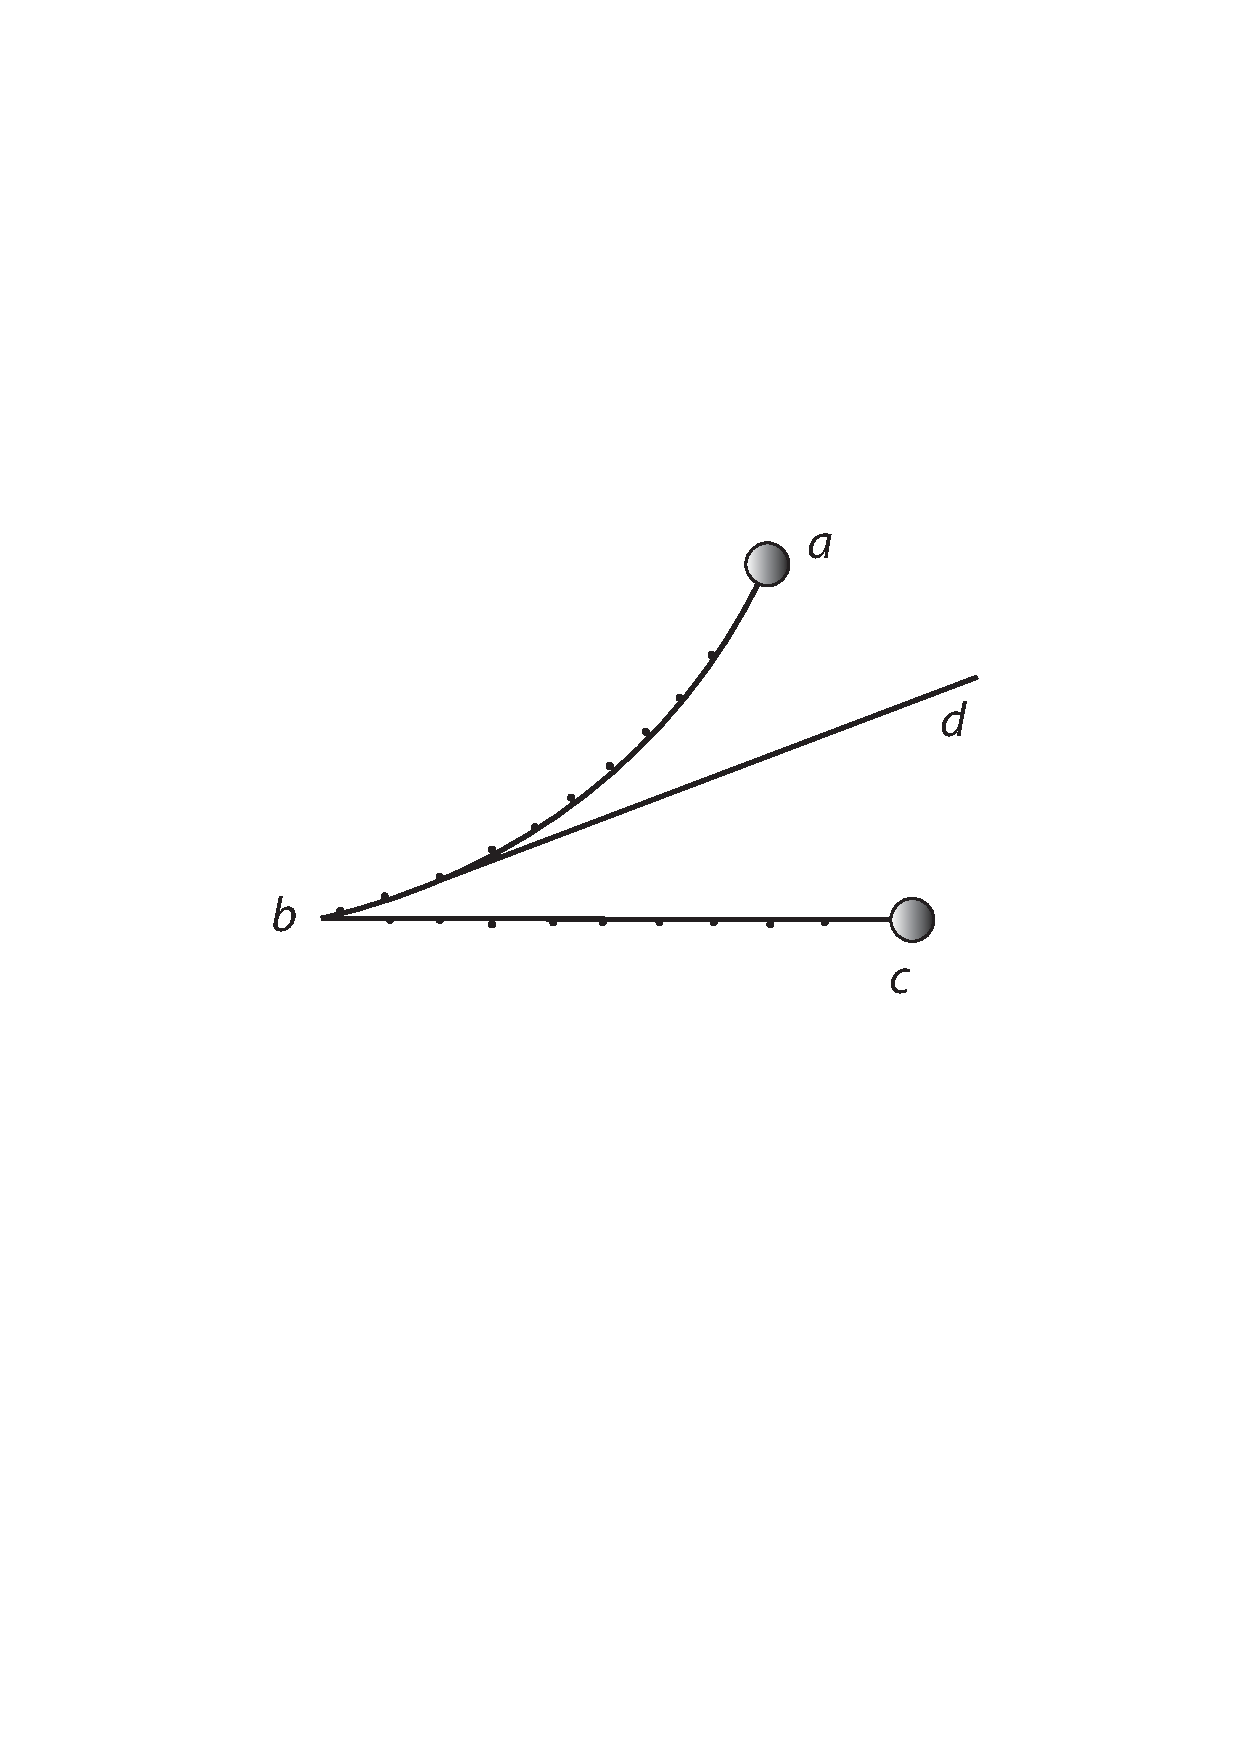
\includegraphics[trim = 0mm 0mm 0mm 0mm, clip, width=0.36\textwidth]{images/lh374_34rkonvertiert.pdf}\\
 \noindent \centering [\textit{Fig. 1}] 
  \pend
 

